% Created 2016-01-14 四 15:20
\documentclass[11pt]{article}
\usepackage[utf8]{inputenc}
\usepackage[T1]{fontenc}
\usepackage{fixltx2e}
\usepackage{graphicx}
\usepackage{longtable}
\usepackage{float}
\usepackage{wrapfig}
\usepackage{rotating}
\usepackage[normalem]{ulem}
\usepackage{amsmath}
\usepackage{textcomp}
\usepackage{marvosym}
\usepackage{wasysym}
\usepackage{amssymb}
\usepackage{hyperref}
\tolerance=1000
\usepackage{xeCJK}
\usepackage{framed} \usepackage{subcaption} \usepackage[section]{placeins} \usepackage{wrapfig}
\author{钱泽森(5130379069)}
\date{\today}
\title{Quidditch桌球详细设计说明书}
\hypersetup{
  pdfkeywords={},
  pdfsubject={},
  pdfcreator={Emacs 24.5.1 (Org mode 8.2.10)}}
\begin{document}

\maketitle
\tableofcontents


\section{引言}
\label{sec-1}
\subsection{编写目的和范围}
\label{sec-1-1}
本详细设计说明书编写的目的是说明程序模块的设计考虑,包括程序描述、
输入/输出、算法和流程逻辑等,为软件编程和系统维护提供基础。本说明书
的预期读者为系统设计人员、软件开发人员、软件测试人员和项目评审人员。
\subsection{术语表}
\label{sec-1-2}
\begin{description}
\item[{Buffer Object}] An object that represents a linear array of
memory, which is stored in the GPU. There are
numerous ways to have the GPU access data in a
buffer object.
\item[{Context, OpenGL}] A collection of state, memory and resources.
Required to do any OpenGL operation.
\item[{OpenGL Shading Language}] The language for writing Shaders in
OpenGL.
\item[{Shader}] A program, written in the OpenGL Shader Language,
intended to run within OpenGL.
\item[{Texture}] An OpenGL object that contains one or more images, all
of which are stored in the same Image Format.
\item[{OpenGL}] A cross-platform graphics system with an openly
available specification.
\end{description}
\subsection{参考资料}
\label{sec-1-3}
\begin{center}
\begin{tabular}{llll}
资料名称 & 作者 & 文件编号/版本 & 资料存放地点\\
OpenGL Tutorial & Unknown & latest & \url{http://www.opengl-tutorial.org}\\
OpenGL step by step & Unknown & Latest & \url{http://ogldev.atspace.co.uk/}\\
OpenGL wiki & collabrators & Latest & \url{https://www.opengl.org/wiki/}\\
OpenGL 3.3 Reference Pages & SGI & 3.3 & \url{https://www.opengl.org/sdk/docs/}\\
Bullet Physics Doc & Bullet & 2.83 & \url{http://bulletphysics.org/Bullet/BulletFull/index.html}\\
\end{tabular}
\end{center}

\subsection{使用的文字处理和绘图工具}
\label{sec-1-4}
\begin{description}
\item[{文字处理软件}] Emacs, Org Mode
\item[{UML图生成}] Doxygen
\end{description}
\section{技术概要}
\label{sec-2}
\begin{itemize}
\item 基于OpenGL 3.3 core API
\item 使用了 SFML 作为window system
\item 使用 glew 作为Extension Wrangler Library
\item 使用glm作为数学库
\item 使用Bullet Physics作为物理引擎
\item 开发环境为Linux x86-64 + Mesa
\end{itemize}
\section{模块设计}
\label{sec-3}
\subsection{控制模块}
\label{sec-3-1}
\subsubsection{沙盒(\texttt{Arena})}
\label{sec-3-1-1}
沙盒模块负责对物理世界进行仿真模拟. 由于本软件已经使用Bullet
Physics作为物理引擎, 因此本软件的着重点在于将Bullet Physics应用到
程序中. \texttt{Arena} 实际上是对Bullet的一个包装. 我们定义了如下几个类.
\subsubsection{控制器(\texttt{Controller})}
\label{sec-3-1-2}
这是一个抽象类, 用来控制游戏世界中的一个(\texttt{SingleController})或者多个
(\texttt{GroupController})实体. 本类中定义了一个虚方法:

\begin{verbatim}
virtual bool control(const float elapsed);
\end{verbatim}

所有继承类都要实现这个虚方法. 在每个时间片的开始, \texttt{Arena} 都会调用这
个方法, elapsed表示距离上次调用已经过去了多少时间. Controller需要
根据自己的用途, 来控制自己所代表的刚体. 这个控制, 既可以是来自用户的(\texttt{CueBall}), 也可以是来自自身的
(\texttt{WanderBall}). 下面对 \texttt{Controller} 最主要的几个子类进行解释.
继承关系请见图\ref{fig:controller_inherit}.

\begin{figure}[h]
\centering
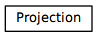
\includegraphics[width=\textwidth]{html/inherit_graph_3.png}
\caption{Controller的继承关系}
\label{fig:controller_inherit}
\end{figure}
\subsubsection{球(\texttt{Ball})}
\label{sec-3-1-3}
所有球类的父类. 主要用于归类, 没有特殊用途.
\subsubsection{幽灵球(\texttt{GhostBall})}
\label{sec-3-1-4}
普通球, 没有任何行为,因此他的 \texttt{control} 方法什么也不做.
\subsubsection{母球(\texttt{CueBall})}
\label{sec-3-1-5}
受用户控制, 每个时间片都会读取用户的键盘输入, 并且对所控制的刚体
球施加一个力.
\subsubsection{游走球(\texttt{WanderBall})}
\label{sec-3-1-6}
自主随机游走的球, 每个时间片都会检查当前的速度和理想速度, 并且
逐渐趋近这个理想速度.
\subsubsection{金色飞贼(\texttt{SnitchBall})}
\label{sec-3-1-7}
会飞的球, 每隔一段时间都会离地飞行, 一段时间后又会落回地面.

\subsubsection{迷球(\texttt{FantasyBall})}
\label{sec-3-1-8}
我为了增加游戏性, 特意增加的一种球, 作为一种惩罚措施. 母球碰到该球
后, 之后一段时间的操作都会被反向地执行.
\subsubsection{桌面(\texttt{Ground})}
\label{sec-3-1-9}
指的是小球运动的桌面. 凹凸不平的地面是由Perlin函数生成的.
\subsection{粒子系统}
\label{sec-3-2}
\label{sec:particle}
为了增加真实性, 我对粒子系统做了如下处理:
\begin{itemize}
\item 每个粒子都是一个正方形的billboard, 也就是说, 我们通过一些计算,
使得该正方形的面始终正对摄像机镜头. 这样做有几个好处: 
\begin{itemize}
\item 减少了一半绘画的面数(否则至少需要一个四面体来保证从各个方向都能看到微粒)
\item 效果更加真实(四面体的微粒不真实).
\end{itemize}
\begin{verbatim}
fragPos = centerPos
  + cameraRight * vert.x * size
  + cameraUp * vert.y * size;
\end{verbatim}
\item 锋利的边缘让微粒看起来很不真实, 因此我在Fragment Shader中做了处
理: 对于同一个微粒, 正中央的alpha最高, 边缘的alpha为零, 中间平
滑过度. 这样子的微粒才有朦胧的感觉. 效果对比请见图\ref{fig:smooth}.
\begin{verbatim}
surfaceColor.a *= 1 - distance(fragPos, centerPos) / size;
\end{verbatim}

\begin{figure}[h]
\centering

\begin{subfigure}[b]{0.4\textwidth}
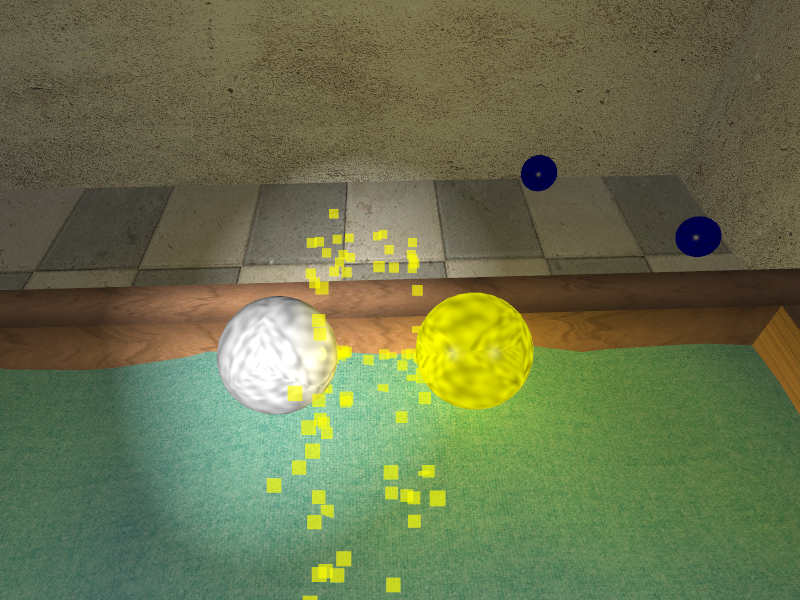
\includegraphics[width=\textwidth]{without-smooth.png}
\caption{Without smooth}
\label{fig:without-smooth}
\end{subfigure}
~
\begin{subfigure}[b]{0.4\textwidth}
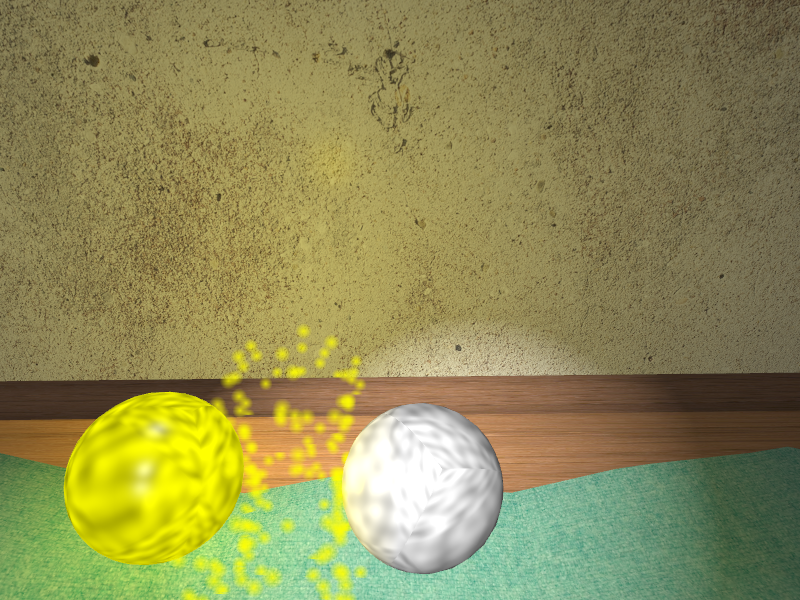
\includegraphics[width=\textwidth]{with-smooth.png}
\caption{With smooth}
\label{fig:with-smooth}
\end{subfigure}

\caption{开启平滑前后对比} \label{fig:smooth}
\end{figure}
\end{itemize}
为了提高性能, 我做了如下优化:
\begin{itemize}
\item 使用了OpenGL提供的Instancing接口. 对于数万个微粒, 如果对于每个
微粒都调用一次OpenGL的绘图函数, Overhead太大, 无法进行实时的流
畅绘画. 因此我采用了OpenGL的Instancing, 对于数万个微粒, 只需要
提供单个微粒的样板(如上所说, 是一个正方形)和每个微粒的位置, 只
需要一次OpenGL的函数调用, 就可以画出数万个微粒, 极大地提高了性能.
\begin{verbatim}
glDrawArraysInstanced(GL_TRIANGLE_STRIP, 0, 4, vertOffset.size());
\end{verbatim}
\end{itemize}

\subsubsection{火花(\texttt{Spark})}
\label{sec-3-2-1}
在白色母球和金色飞贼碰撞时触发. 包含数千个微粒, 在这里我使用了Bullet
来模拟火花的行为, 理由如下:
\begin{itemize}
\item 火花会收到重力的影响, 应该放到物理系统里模拟.
\item 火花会和别的物体碰撞, 这一点也应该放到物理系统来模拟. 一个意外
的收获是, 只要每个火花的质量不太小, 火花能够对周围的物体产生可
见的影响, 我利用这一点, 使得白色母球和金色飞贼在碰撞后会像触电
一样弹开.
\end{itemize}

另外我做了一个小细节, 使得每个时间周期都会对每个火花的颜色做调整(逐渐变暗), 使得火花
在整个生命周期中显现出一种"逐渐熄灭"的感觉. 
\subsubsection{烟雾(\texttt{Smoke})}
\label{sec-3-2-2}
从迷球表面散发, 用来警告用户. 包含数万个微粒.

为了追求真实性, 在离子系统的通用优化的基础上, 我进一步做了如下处理:
\begin{itemize}
\item 每个微粒都有一个生命周期, 在这个生命周期内, 他的alpha(不透明度
)会逐渐减小直到变成零, 然后被删除.  这种做法比较好的模拟了烟雾逐
渐消散的过程. 效果对比请见图\ref{fig:fadeout}.
\end{itemize}

\begin{figure}[h]
\centering

\begin{subfigure}[b]{0.4\textwidth}
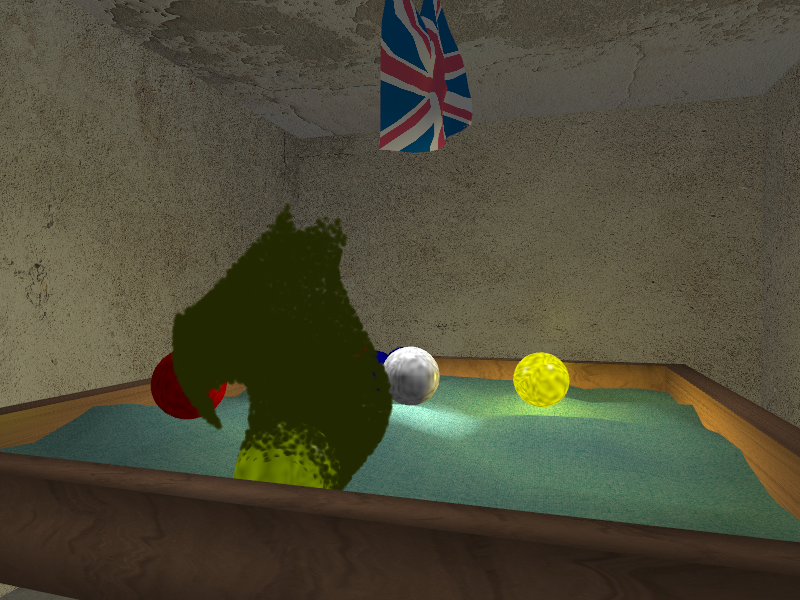
\includegraphics[width=\textwidth]{without-fadeout.png}
\caption{Without Fadeout}
\label{fig:without-fadeout}
\end{subfigure}
~
\begin{subfigure}[b]{0.4\textwidth}
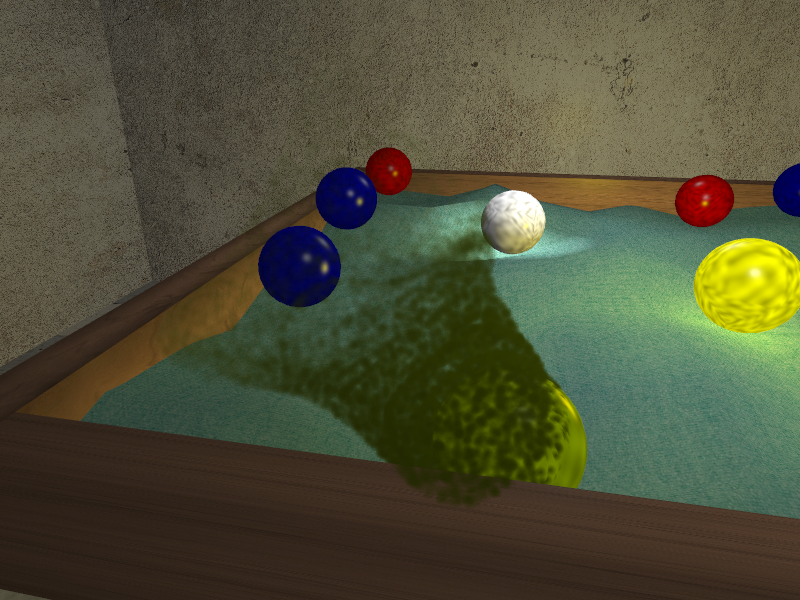
\includegraphics[width=\textwidth]{with-fadeout.png}
\caption{With fadeout}
\label{fig:with-fadeout}
\end{subfigure}

\caption{开启渐变前后对比} \label{fig:fadeout}
\end{figure}

为了提高性能, 在粒子系统的通用优化的基础上, 我做了如下优化:
\begin{itemize}
\item 不使用Bullet Physics的物理系统来模拟微粒的运动, 而使用噪声函数
来仿真. 为了真实性, 我们的微粒数量应该尽可能多, 以数万为最佳. 经过测试, Bullet在这种数
量级的物体下, 无法进行实时的流畅模拟. 因此我放弃了纯物理的方式,
转而投向了噪声函数模拟. 在这里我们复用了Perlin函数, 来生成每个
微粒在下一个时间片的速度. 噪声的参数是绝对时间和小球的绝对方位. 这
样可以保证烟雾在时间和空间上都保持连续, 但是都保持逐渐变化.
\end{itemize}
\subsection{软体系统}
\label{sec-3-3}
\subsubsection{布料(\texttt{Cloth})}
\label{sec-3-3-1}
本质上是一个长方形的Mesh, 包含数百个小三角形. 相邻的几个节点之间会
有link相连, 来限制他们的相对运动. 
关于风的模拟: 在每一个时间片中, 对于该软体的每个节点, 都从一个噪声
函数生成一个受力. 这个噪声函数的参数是该节点的绝对位置和当前绝对时
间. 这样既保证了受力在时间和空间上的连续性, 又保证了一定的变化.
\subsection{绘图模块}
\label{sec-3-4}
\subsubsection{场景(\texttt{Scene})}
\label{sec-3-4-1}
表示一个完整的场景, 包括一些 \texttt{Render}, \texttt{Light}, \texttt{Particle}.
\subsubsection{可渲染物体(\texttt{Render})}
\label{sec-3-4-2}
是一个抽象类, 只是定义了一个通用接口, 调用后即会画出该物体, 所有的
继承类都要实现该接口. 
\begin{verbatim}
virtual void render(ModelSetter ms, MaterialSetter ts) const = 0;
\end{verbatim}
\texttt{ModelSetter} 是一个回调函数, 来设定这个物体在全局中位置.
\texttt{MaterialSetter} 也是一个回调函数, 来设定这个物体的材料. 材料的定
义包括:
\begin{itemize}
\item 纹理
\item 反光度
\item 反光的颜色
\item 自发光亮度
\end{itemize}

继承关系请见图\ref{fig:render_inherit}.

\begin{figure}[h]
\begin{center}
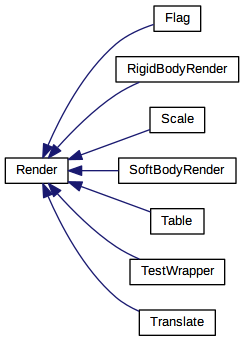
\includegraphics[width=0.5\textwidth]{html/inherit_graph_20.png}
\end{center}
\caption{Render的继承关系}
\label{fig:render_inherit}
\end{figure}
\subsubsection{形状(\texttt{Shape})}
\label{sec-3-4-3}
也是一个抽象类, 定义了一个通用接口, 调用后即会画出该物体. 
\begin{verbatim}
virtual void render(Render::ModelSetter ms) const = 0;
\end{verbatim}
其中 \texttt{ModelSetter} 是一个回调函数, 来设定这个物体在全局中位置.
继承关系请见图\ref{fig:shape_inherit}.

\begin{figure}[h]
\centering
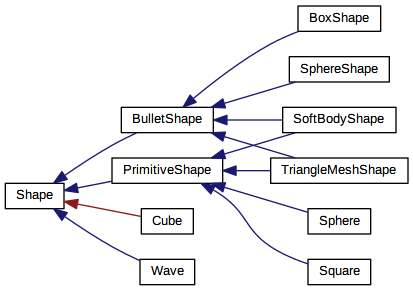
\includegraphics[width=0.8\textwidth]{html/inherit_graph_23.png}
\caption{Shape的继承关系}
\label{fig:shape_inherit}
\end{figure}

下面着重讲一下 \texttt{Sphere} (球)的实现方法.
\begin{enumerate}
\item 球(Sphere)
\label{sec-3-4-3-1}
\begin{figure}[h]
\centering
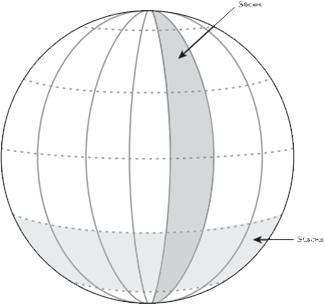
\includegraphics[width=0.50\textwidth]{gluSphere.png}
\caption{gluSphere的划分方式}
\label{fig:gluSphere}
\end{figure}

大多数人都会选择使用 \texttt{gluSphere} 函数(见图\ref{fig:gluSphere})来直接生成球体, 但是我认为这
种方法有如下缺陷:
\begin{itemize}
\item 划分不均匀, 在两极点的划分明显要比赤道的划分密得多. 为了达到某
个划分细度, 则必须要在赤道达到该密度, 则此时极点的密度是过高的,
造成了绘图资源的浪费.
\item 难以复用. 对于每一个球体, 用户都需要调用 \texttt{gluSphere} 来绘出这一
个球体. 这至少造成了两方面的浪费. 一是每次调用都需要重新计算每
个节点的坐标, 造成了cpu资源的浪费. 二是每个球体都需要把节点坐标
传到GPU中, 造成了GPU带宽和GPU Memory的浪费.
\end{itemize}

\begin{figure}[h]
\centering
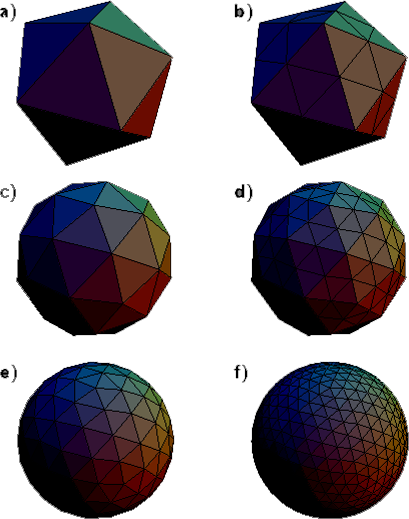
\includegraphics[width=0.48\textwidth]{sphere.png}
\caption{更好的划分方式}
\label{fig:sphere}
\end{figure}

由于这些原因, 我没有采用这种简单的办法, 而是用三角形剖分的方式来
生成球形(见图\ref{fig:sphere}). 方法如下:
\begin{enumerate}
\item 首先生成一个正四面体.
\item 对于四面体的每个三角面, 均匀分成四个三角面.
\item 将新生成的节点, 延长到球体的表面上.
\item 重复2,3步骤, 直到足够的精度为止.
\end{enumerate}

实际使用过程中, 我大概需要迭代3次, 也就是说, 大约256个面的球
体, 已经非常细腻了. 这一方法完美解决了上面提到的问题.
\end{enumerate}
\subsubsection{光照(\texttt{Light})}
\label{sec-3-4-4}
在Phong的光照模型上, 做了几个改进:
\begin{itemize}
\item 加了自发光系数, 来保证发光物体看起来是亮的.
\item 加了衰减系数, 使得较远的物体看起来较暗.
\item 加了光照方向, 来支持聚光灯.
\end{itemize}
\begin{verbatim}
struct Spec {
  glm::vec4 position; //光源位置
  glm::vec3 intensities; //光色
  float attenuation; //衰减系数
  float ambientCoefficient; //环境光照系数
  glm::vec3 coneDirection; //光照方向
  float coneAngle; //方向角宽
};
\end{verbatim}
继承关系请见图\ref{fig:light_inherit}.

\begin{figure}[h]
\centering
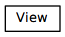
\includegraphics[width=0.48\textwidth]{html/inherit_graph_8.png}
\caption{Light的继承关系}
\label{fig:light_inherit}
\end{figure}
\begin{description}
\item[{FollowSpotlight}] 也就是聚光灯, 会跟随某个物体移动.
\item[{MovingLight}] 依附在某个物体上的灯, 主要用来支持自发光物体, 比
如金色飞贼
\item[{SimpleLight}] 最简单的的灯, 所有系数都是固定的.
\item[{ToggleLight}] 支持开关的灯.
\end{description}
\subsubsection{粒子系统(\texttt{Particle})}
\label{sec-3-4-5}
请见\ref{sec:particle}.
\subsubsection{视角(\texttt{View})}
\label{sec-3-4-6}
表示用户的视角, 包括摄像头所在的位置, 观察的方向等等, 可以调用获
取对应的View Matirx.

\subsubsection{投影(\texttt{Projection})}
\label{sec-3-4-7}
表示摄像头的投影, 包括横向的和纵向的视角, 最近的切点和最远处的切
点, 可以调用获取对应的Projection Matrix.

\subsection{音效系统}
\label{sec-3-5}
我实现了一个立体声的音效系统, 实现方法如下:
\begin{itemize}
\item 维护一个向量来表示玩家视角当前的位置, 一个向量表示玩家当前的朝向.
\item 对于场景中产生的某次碰撞或其他事件, 根据多个因素,来决定双声道中音量的大小. 总的来说, 具体的音效播放与下列因素均有关系:
\begin{itemize}
\item 玩家所在的位置, 和面对的方向
\item 音效所在的位置
\item 该事件的烈度, 比如碰撞时产生的弹力大小
\end{itemize}
\end{itemize}
目前我对球与球之间的碰撞, 以及球与挡板之间的碰撞, 均做了碰撞的音效.
% Emacs 24.5.1 (Org mode 8.2.10)
\end{document}